\documentclass{article}

% Camera-ready: named authors visible
\usepackage[dblblindworkshop, final]{neurips_2026}
\workshoptitle{NeurIPS 2026 Workshop VerifyAgents}

\usepackage[utf8]{inputenc}
\usepackage[T1]{fontenc}
\usepackage{hyperref}
\usepackage{url}
\usepackage{booktabs}
\usepackage{amsfonts}
\usepackage{nicefrac}
\usepackage{microtype}
\usepackage{xcolor}
\usepackage{graphicx}
\usepackage{amsmath}

\title{Reliability \& Fallback Design Patterns for Multi-Agent LLM Systems}

\author{%
  Muhammad Ashar Ishfaq \\
  The Islamia University of Bahawalpur
  \And
  Muhammad Asad Ishfaq \\
  Indiana University Bloomington
}

\begin{document}

\maketitle

\begin{abstract}
We present an empirical side-by-side comparison of orchestration-level fallback strategies---not new algorithms---on a fixed multi-agent QA pipeline. On 150 HotpotQA questions $\times$ three trials (450 logged runs per condition), we compare two baselines (no fallback, blind retry) against four targeted recovery patterns and one tested composition (P1$+$P2), reporting pass rate, p95 latency, and cost together. Targeted fallbacks that address \emph{common recoverable failure modes} in our Claude Sonnet testbed (especially schema/JSON breakage) significantly beat no fallback under question-level McNemar tests with Bonferroni correction (P1/P2/P3/P5 vs.\ B0: each $p < 10^{-6}$). Blind retry does not ($p{=}0.0265$, n.s.\ after correction). P4 also beats B0 ($p{=}7.2\times 10^{-5}$) but is worse than P3 on pass rate at $2.5\times$ the cost ($p{=}5.1\times 10^{-4}$ for P3 vs.\ P4). The tested P1$+$P2 composition does not beat the best single targeted pattern ($p{=}0.37$ vs.\ P1). A GPT-4o-mini probe on the same question IDs shows no significant lift when structural failures are rare---so gains are conditional on the baseline error profile, not universal. We release code, data, and logs.
\end{abstract}

\section{Introduction}
\label{sec:intro}

Multi-agent LLM pipelines fail mid-run: bad sub-questions, empty retrieval, broken JSON, or ungrounded citations. Agent frameworks and production stacks commonly expose \emph{retry loops} or halt on error---Reflexion-style verbal retry~\citep{shinn2023reflexion}, self-consistency sampling~\citep{wang2023selfconsistency}, and targeted re-roll after diagnosis~\citep{zhu2025agentdebug}---but rarely compare orchestration policies on \emph{end-to-end} failure, latency, and cost under identical workloads.

\textbf{Contribution.} We do not propose new fallback algorithms. We benchmark seven fixed conditions on the same 150 HotpotQA questions~\citep{yang2018hotpotqa} and corpus in a Planner--Retriever--Synthesizer--Formatter LangGraph pipeline: \textbf{baselines} B0 (no fallback) and B1 (blind retry), \textbf{vs.\ four targeted patterns} P1--P4 (tool-grounded retry, checkpointing, degradation, cross-agent verification) and one \textbf{tested composition} P5 (P1 then P2). Prior work validates individual techniques (CRITIC-style tool critique~\citep{gou2024critic}, cascades~\citep{chen2024frugalgpt}, debate~\citep{du2024debate}); what was missing is a multi-objective menu under one testbed---including whether stacking two targeted patterns beats either alone.

\textbf{Headline findings (Claude Sonnet, this testbed).} Targeted fallbacks beat B0 when they match prevalent recoverable failures (here, largely \texttt{broken\_json}; McNemar on 150 paired questions, Section~\ref{sec:results}). Blind retry does not ($p{=}0.0265$ vs.\ B0, n.s.\ after Bonferroni) and stretches p95 latency. P4 beats B0 ($p{=}7.2\times 10^{-5}$) but trails P3 on pass rate at higher cost. P5 (the only composition we test) does not add significant gain over P1 ($p{=}0.371$). On GPT-4o-mini, B0/P1/P3 are 69\%/68\%/71\% (n.s.)---gains are \emph{failure-mode-dependent}, not universal.

Section~\ref{sec:related} situates prior work. Sections~\ref{sec:method}--\ref{sec:setup} describe the pipeline and statistics. Section~\ref{sec:results} reports pooled metrics with question-level significance tests. Appendix~\ref{app:extra} holds ablations, failure types, 2WikiMultihopQA, and the GPT-4o-mini table.

\section{Related Work}
\label{sec:related}

Much LLM reliability work is try-again: Self-Consistency~\citep{wang2023selfconsistency} votes over samples; Reflexion~\citep{shinn2023reflexion} retries with verbal memory; CRITIC~\citep{gou2024critic} revises using tool signals. Intrinsic self-correction without external feedback often fails~\citep{huang2024cannot,kamoi2024survey}, motivating our tool/schema checks. FrugalGPT~\citep{chen2024frugalgpt} budgets cost and quality via cascades but not mid-graph orchestration fallbacks. Multiagent Debate~\citep{du2024debate} and LLM-as-judge~\citep{zheng2023judge} sit in the same tradeoff space as P4. Production RCA~\citep{tan2026llrca,roy2024rca} diagnoses deployed systems after the fact. Agent surveys~\citep{wang2024agentsurvey,song2026failures} map failure modes; AgentDebug~\citep{zhu2025agentdebug} shows targeted re-roll can beat undifferentiated retry for one mechanism. Few works report failure rate, p95 latency, and dollar cost on the same runs for several orchestration fallbacks on one multi-agent testbed.

\section{Method}
\label{sec:method}

\subsection{Testbed}
Four stages: \textbf{Planner}, \textbf{Retriever}, \textbf{Synthesizer}, \textbf{Formatter}. Retriever searches a fixed local Hotpot-derived corpus (no live web). LLM stages use Claude Sonnet (\texttt{claude-sonnet-4-6}) at temperature 0, except P3's rare Haiku path. Typed shared state exposes stage failures to fallbacks. Success is a scored-correct final answer (Section~\ref{sec:setup}).

\subsection{Conditions}
Seven conditions represent structurally distinct recovery mechanisms---not an exhaustive design-space search; self-consistency and debate are related but distinct (Section~\ref{sec:related}).

\textbf{B0 --- No fallback.} One pass; hard error or wrong final answer counts as failure.

\textbf{B1 --- Blind retry.} Re-run failing stage/graph up to a cap with the same prompts/tools; no new evidence or rollback.

\textbf{P1 --- Tool-grounded retry.} External checks (retrieval, citation IDs, JSON schema); capped stage re-run with check feedback.

\textbf{P2 --- Deterministic checkpointing.} Restore last trusted checkpoint and re-execute forward after failure.

\textbf{P3 --- Graceful degradation.} Simplify path (e.g., skip planning, Haiku cascade) after repeated failure or budget exhaustion.

\textbf{P4 --- Cross-agent verification gate.} Second Verifier agent before formatting; one capped Synthesizer re-run on reject.

\textbf{P5 --- Composed P1$+$P2.} P1 tool-grounded retry first; on continued failure, P2 checkpoint rollback (cap 2 retries/stage). Most questions recover within P1's capped checks and never enter the checkpoint branch; when they do, rollback avoids stacking the long blind-retry chains that inflate B1's tail, which helps explain P5's lower p95 than P1 despite extra orchestration logic.

P1--P3 and P5 use external signals rather than intrinsic self-correction~\citep{huang2024cannot,kamoi2024survey}; P4 is an LLM judge.

\section{Experimental Setup}
\label{sec:setup}

\textbf{Dataset.} 150 HotpotQA distractor validation questions~\citep{yang2018hotpotqa} (short gold; bridge-preferred filters). Corpus: 300 supporting + 20 distractor documents; retriever searches only this set.

\textbf{Scoring.} Normalized token-coverage against gold (exact, substring, or gold-token coverage). We do not run a separate semantic-equivalence or factuality judge on the main metric; paraphrases can fail and citation quality is not scored directly (Section~\ref{sec:limitations}). All conditions share the same scorer.

\textbf{Trials.} Three independent trials on the same 150 questions (450 logged runs per condition). Pass rates, Wilson 95\% CIs, latency, and cost in Table~\ref{tab:pooled} and Figures~\ref{fig:pass}--\ref{fig:latency} pool all 450 runs per condition.

\textbf{Inferential testing.} Because the three trials reuse the same 150 questions, run-level outcomes are not independent. All primary pass-rate significance tests are therefore performed at the question level: for each condition and question, we label pass if a \emph{majority} of that question's trials pass, yielding 150 paired binary outcomes per condition pair. We apply two-sided McNemar's test (with continuity correction) and Bonferroni correction over 21 condition pairs ($\alpha{=}0.05/21{=}0.002381$). Table~\ref{tab:pairwise} reports $\Delta$pp and Cohen's $h$ on these question-level majority rates.

\textbf{Metrics.} Pass rate, end-to-end latency (p50/p95), average cost per question.

\section{Results}
\label{sec:results}

\subsection{Headline}
Table~\ref{tab:pooled} summarizes pooled runs (450 per condition). Table~\ref{tab:pairwise} lists McNemar tests on 150 paired questions. P1, P2, P3, and P5 each beat B0 with $p < 10^{-6}$. B1 does not ($p{=}0.0265$, n.s.\ after Bonferroni). P4 beats B0 ($p{=}7.2\times 10^{-5}$) but loses to P3 ($p{=}5.1\times 10^{-4}$) at $2.5\times$ the cost.

\begin{table}[t]
  \caption{Pooled results across three trials (450 runs per condition). Pass\% pools all runs; inferential tests use 150 paired questions (Table~\ref{tab:pairwise}).}
  \label{tab:pooled}
  \centering
  \small
  \begin{tabular}{lrrrrr}
    \toprule
    Cond & Runs & Pass\% & p50 (ms) & p95 (ms) & \$/q \\
    \midrule
    B0 & 450 & 55.3 & 6440 & 11180 & 0.0052 \\
    B1 & 450 & 61.1 & 6889 & 30793 & 0.0085 \\
    P1 & 450 & 76.0 & 7951 & 20528 & 0.0072 \\
    P2 & 450 & 76.2 & 8047 & 18444 & 0.0073 \\
    P3 & 450 & 78.2 & 7764 & 18444 & 0.0073 \\
    P4 & 450 & 68.2 & 12366 & 33553 & 0.0183 \\
    P5 & 450 & 74.7 & 7321 & 12338 & 0.0071 \\
    \bottomrule
  \end{tabular}
\end{table}

\begin{table}[t]
  \caption{Selected pairwise tests on 150 Hotpot questions (majority pass per question; McNemar; Bonferroni $\alpha{=}0.002381$).}
  \label{tab:pairwise}
  \centering
  \small
  \setlength{\tabcolsep}{3.5pt}
  \begin{tabular}{lrrrr}
    \toprule
    Comparison & $\Delta$pp & $p$ & Cohen's $h$ & sig \\
    \midrule
    P1 vs B0 & $+21.3$ & $1.06\times 10^{-7}$ & $0.45$ & ** \\
    P2 vs B0 & $+20.7$ & $8.14\times 10^{-7}$ & $0.44$ & ** \\
    P3 vs B0 & $+24.0$ & $5.43\times 10^{-9}$ & $0.52$ & ** \\
    P5 vs B0 & $+19.3$ & $4.93\times 10^{-7}$ & $0.41$ & ** \\
    P4 vs B0 & $+14.7$ & $7.23\times 10^{-5}$ & $0.30$ & ** \\
    B1 vs B0 & $+6.0$  & $0.0265$ & $0.12$ & ns \\
    P3 vs P1 & $+2.7$  & $0.134$ & --- & ns \\
    P5 vs P1 & $-2.0$  & $0.371$ & --- & ns \\
    P4 vs P3 & $-9.3$  & $5.12\times 10^{-4}$ & --- & ** \\
    \bottomrule
  \end{tabular}
\end{table}

\subsection{Pass rate, cost, and latency}
Figure~\ref{fig:pass} shows pooled pass rates with Wilson 95\% CIs (450 runs). B0 55.3\%; P1--P3/P5 74.7\%--78.2\%; B1 61.1\%; P4 68.2\%. P5 is not significantly above P1 ($p{=}0.371$): we find \emph{no additional benefit from the tested P1$+$P2 composition} (we did not evaluate other compositions).

\begin{figure}[t]
  \centering
  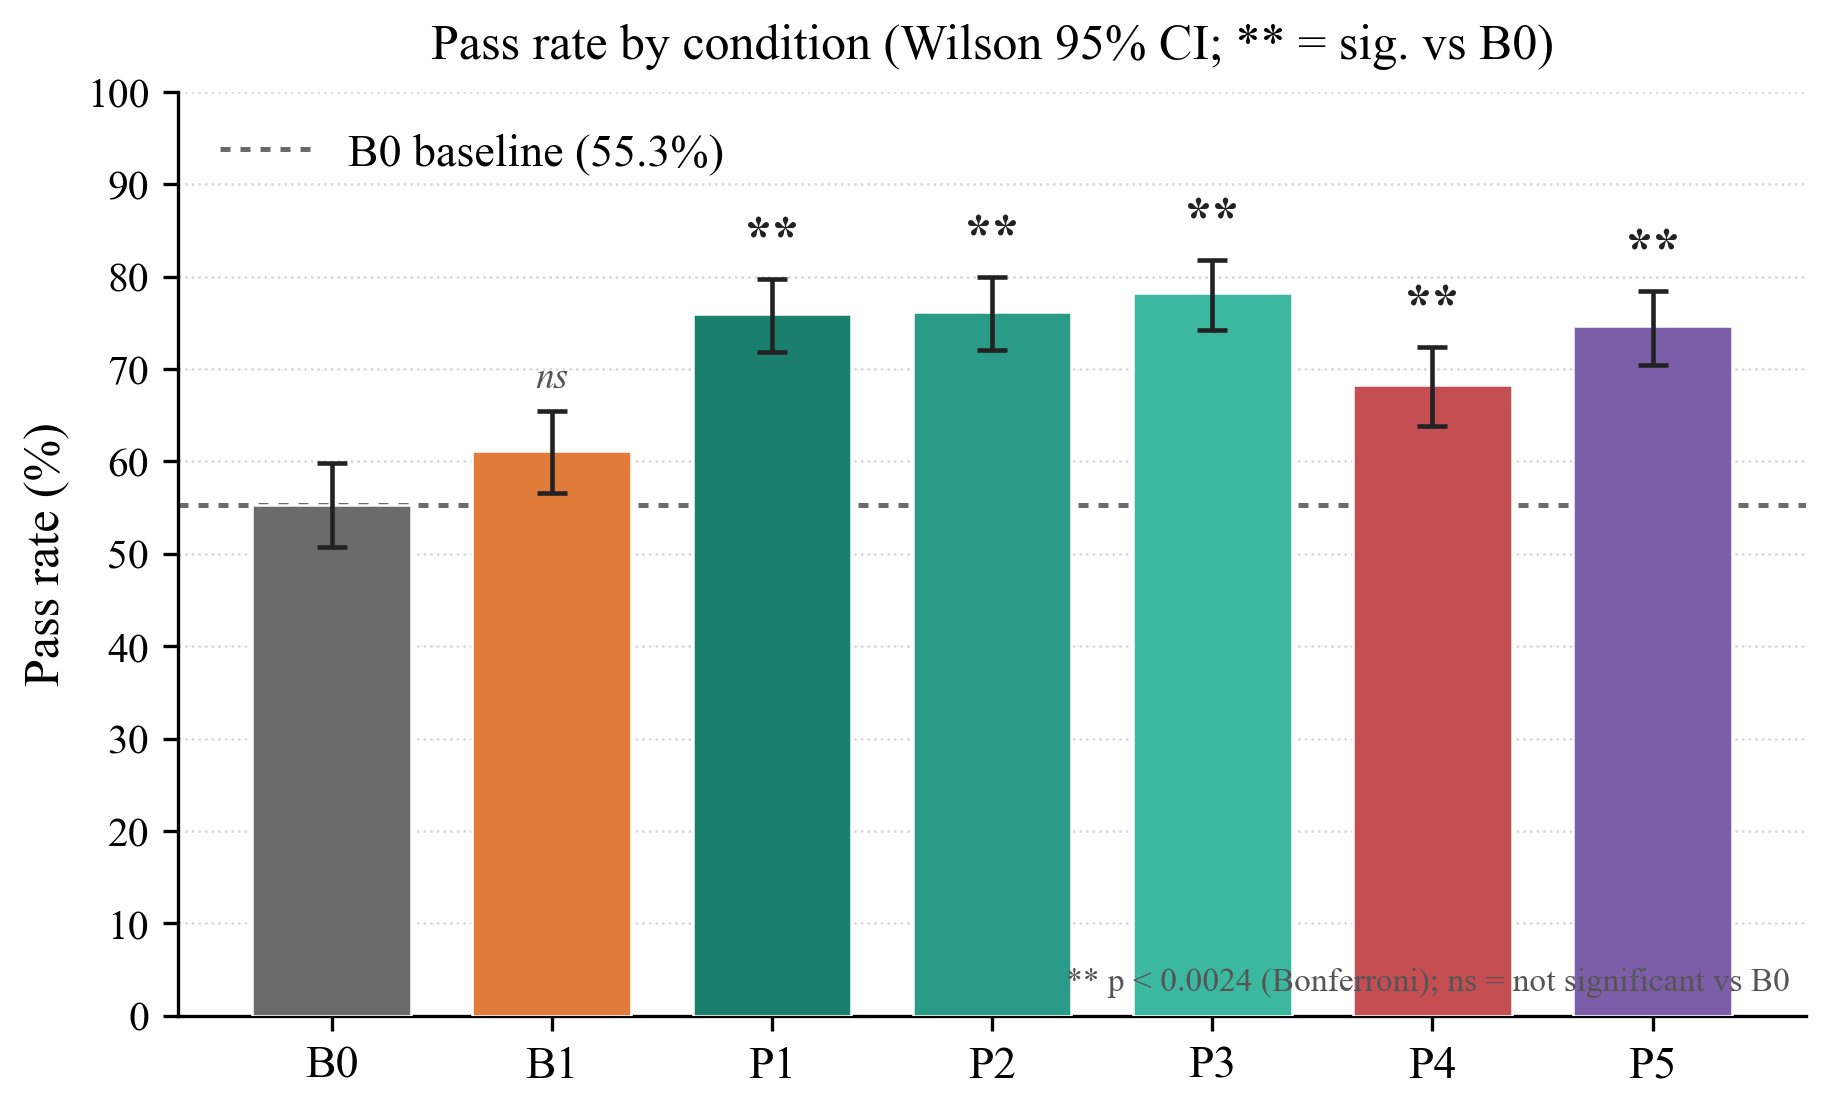
\includegraphics[width=0.88\linewidth]{figures/fig1_pass_rate.png}
  \caption{Pooled pass rate with Wilson 95\% CIs. Markers vs.\ B0: McNemar on 150 paired questions, Bonferroni $\alpha{=}0.002381$.}
  \label{fig:pass}
\end{figure}

Figure~\ref{fig:pareto} (cost vs.\ accuracy) and Figure~\ref{fig:latency} (p95 latency) show the P1--P3/P5 cluster near \$0.007/q with strong pass rates, while B1 and P4 pay more for weaker accuracy and longer tails.

\begin{figure}[t]
  \centering
  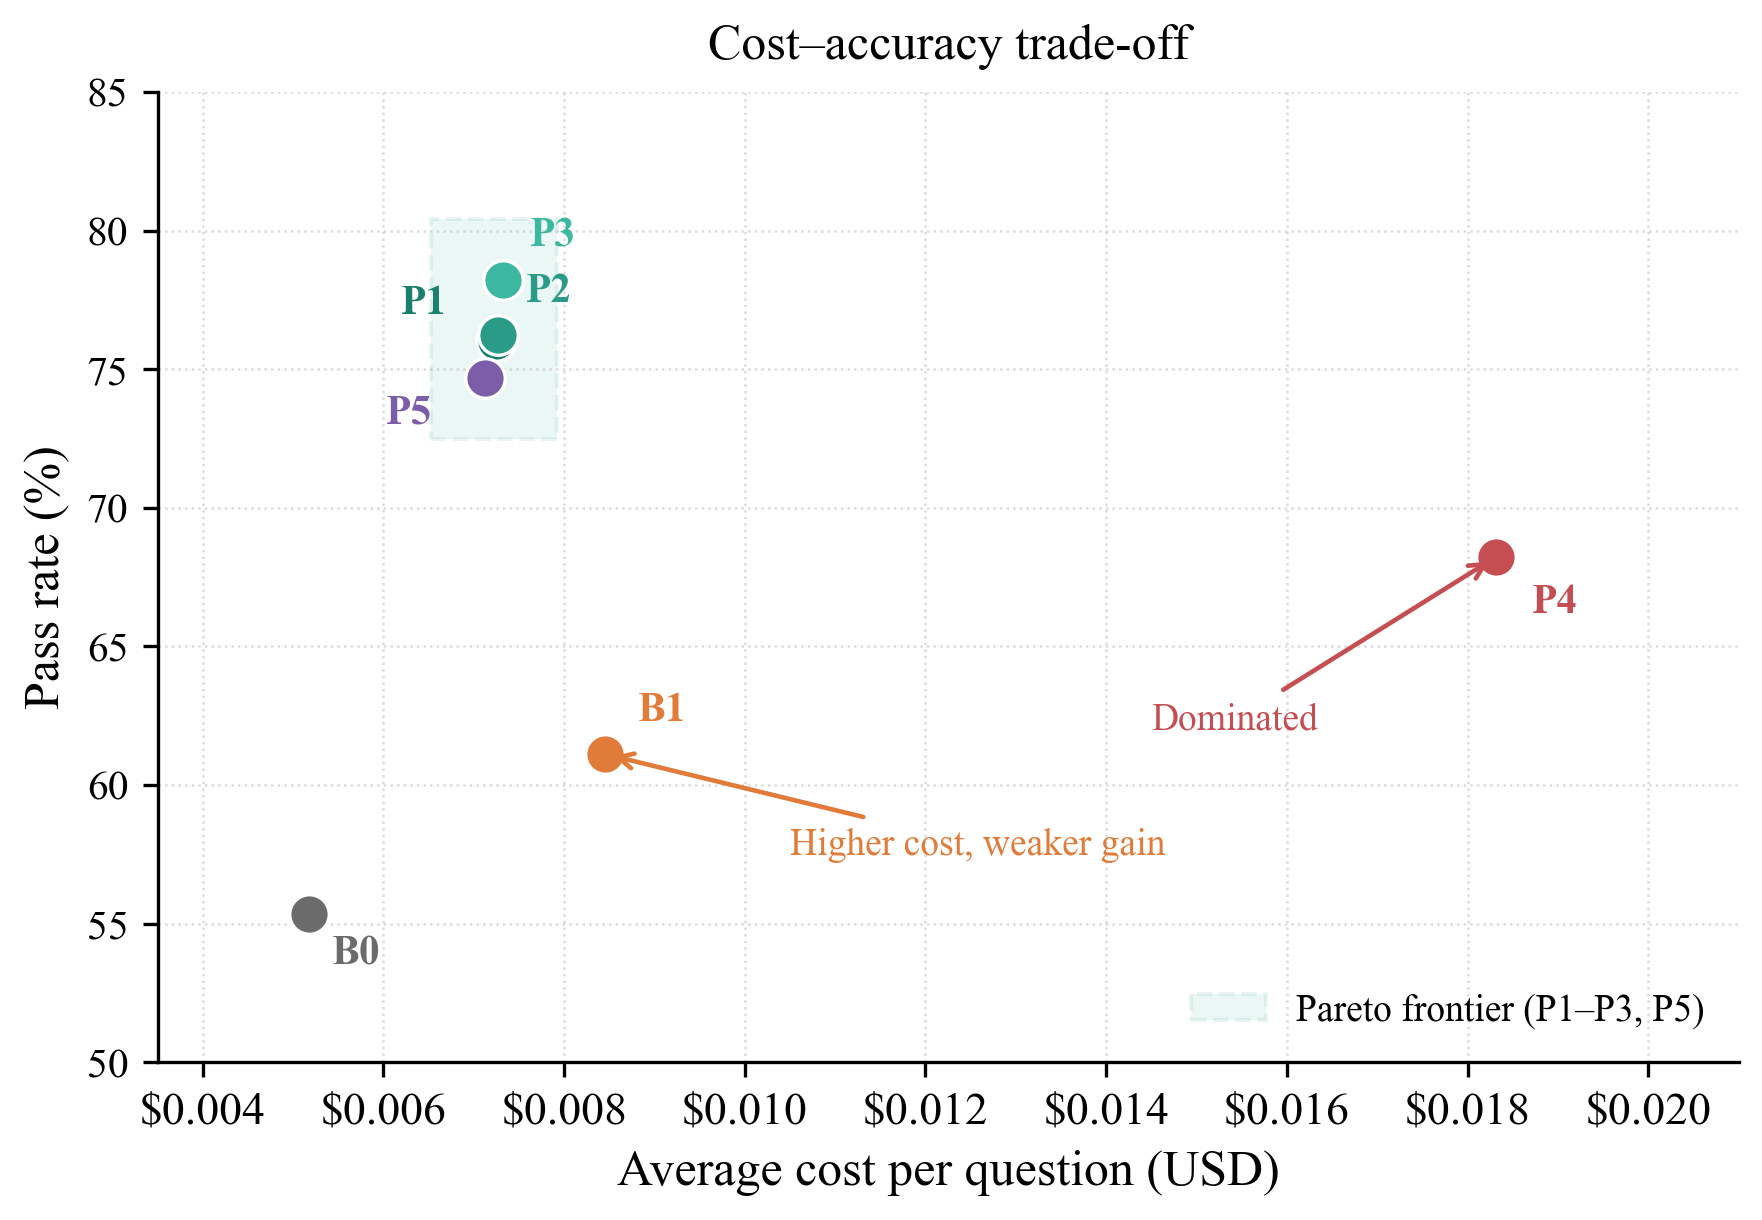
\includegraphics[width=0.88\linewidth]{figures/fig2_cost_accuracy.png}
  \caption{Cost vs.\ accuracy. Dashed box: P1--P3/P5 cluster.}
  \label{fig:pareto}
\end{figure}

\begin{figure}[t]
  \centering
  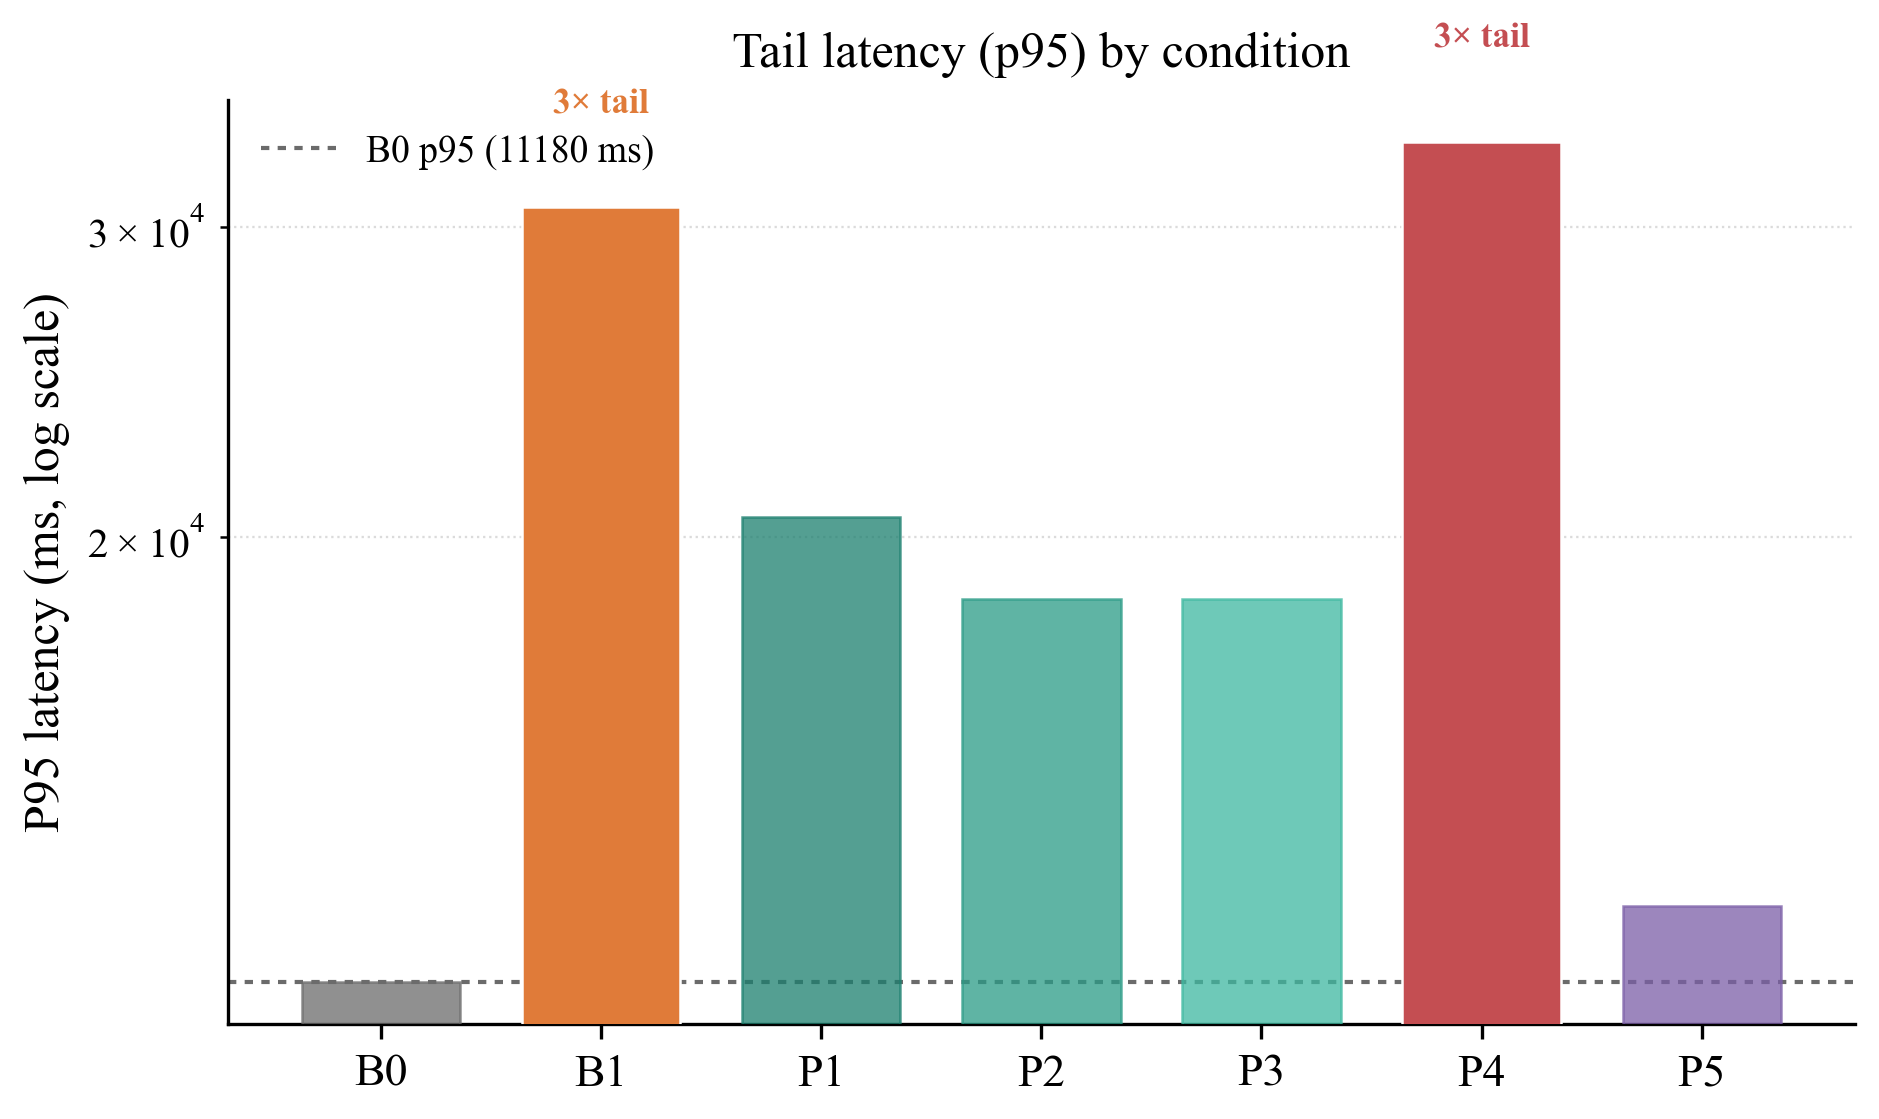
\includegraphics[width=0.88\linewidth]{figures/fig3_latency.png}
  \caption{Pooled p95 latency (log scale). B1 and P4 stretch the tail vs.\ B0.}
  \label{fig:latency}
\end{figure}

\subsection{Composition, stages, and P4}
P5 does not significantly outperform P1/P2/P3 ($p > 0.13$ among targeted cluster). P1--P3 shift failures from Synthesizer to Formatter (Appendix~\ref{app:extra}, Figure~\ref{fig:stage}). P4's verifier false-accept rate is 23.6\% (Figure~\ref{fig:p4conf}), explaining weak cost--reliability tradeoffs despite significance vs.\ B0.

\begin{figure}[t]
  \centering
  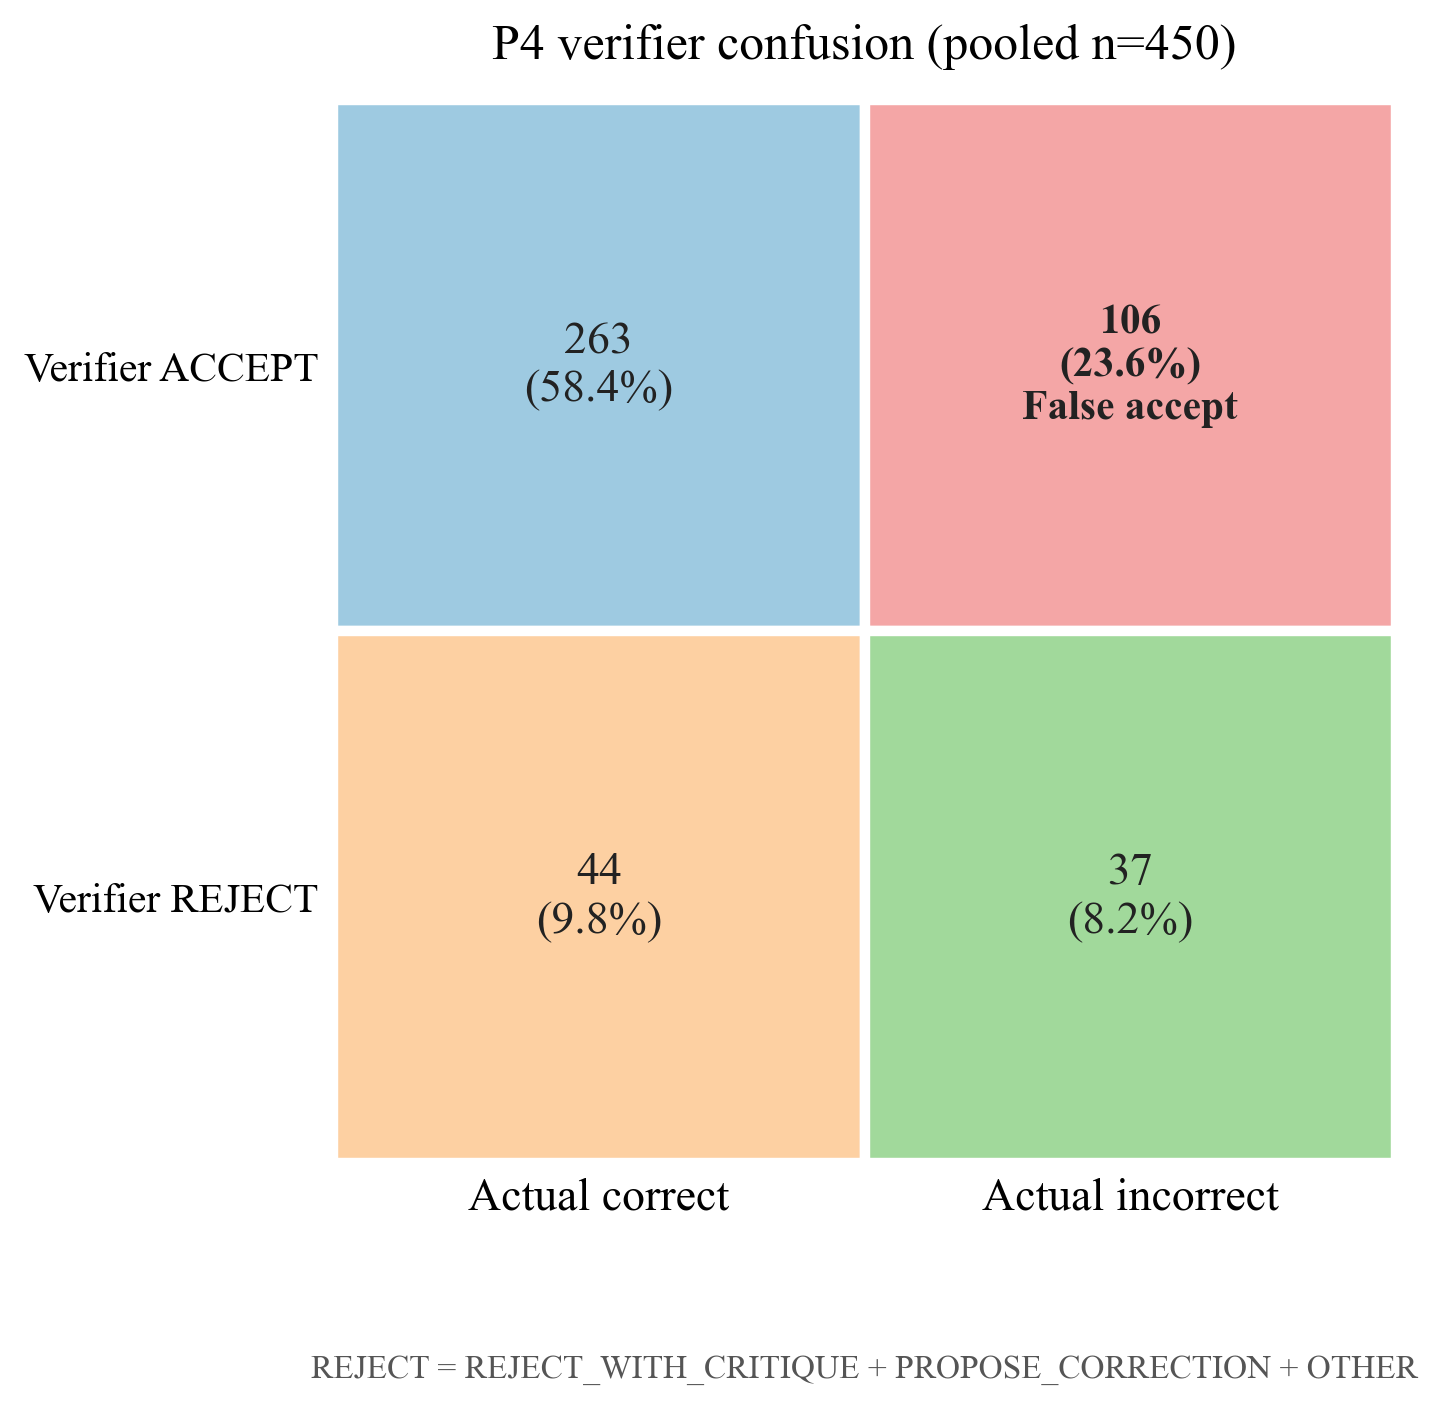
\includegraphics[width=0.62\linewidth]{figures/fig5_p4_confusion.png}
  \caption{P4 verifier confusion (450 pooled runs). False accepts: 23.6\%.}
  \label{fig:p4conf}
\end{figure}

\section{Discussion}
\label{sec:discussion}

Choose fallbacks to match \emph{observed} failure modes. On Claude Sonnet here, schema/JSON checks recover large structural mass; on GPT-4o-mini (Appendix), the same checks barely move pass rate when that mass is absent. Do not default to blind retry (n.s.\ vs.\ B0 after correction; heavy p95). Do not assume a verifier gate is automatically safer: P4 is significant vs.\ B0 ($p{=}7.2\times 10^{-5}$) but has lower pass rate and higher cost than P3 ($p{=}5.1\times 10^{-4}$ for P3 vs.\ P4).

Tool/schema checks with capped retry (P1), checkpoint rollback (P2), degrade (P3), or the tested P1-then-P2 composition (P5) cluster near \$0.007/q with much better pass rates than B0. Reliability looks like orchestration hygiene---external checks, checkpoints, degrade paths---not ``add another agent.''

\paragraph{Reproducibility.}
Code, analysis scripts, and logs: \url{https://github.com/Ashar086/llm-fallback-reliability}.

\section{Limitations}
\label{sec:limitations}

\textbf{Scope.} One primary model family (Claude Sonnet; Haiku on P3's rare path), one main benchmark (150 unique HotpotQA questions), one pipeline topology. Gains on Claude are strongly driven by structural failures (\texttt{broken\_json}); GPT-4o-mini weakens generalization (Appendix).

\textbf{Statistics.} We report pooled 450-run descriptives but test significance on 150 paired questions; trials are not independent.

\textbf{Scoring.} Token-coverage gold matching is brittle; automated semantic equivalence or factuality scoring is future work.

\textbf{Composition.} Only P1$+$P2 was composed; other stacks may differ.

\textbf{Failure taxonomy.} Covers structural/content failures in this testbed, not infrastructure failures (timeouts, rate limits, API outages, vector-DB failures).

\section*{Acknowledgments and Disclosure of Funding}
This work received no external funding.

\bibliographystyle{plainnat}
\bibliography{references}

\appendix
\section{Additional analyses}
\label{app:extra}

\subsection{P1 check ablation}
\label{sec:p1-ablation}
P1 combines retrieval, citation, and schema checks. One-check ablations on 50 Hotpot questions $\times$ two trials ($n{=}100$ runs per variant):

\begin{table}[t]
  \caption{P1 check ablation ($n{=}100$ runs). Wilson 95\% CIs; $z$-tests vs.\ full P1 and B0 on same IDs.}
  \label{tab:p1-ablation}
  \centering
  \small
  \setlength{\tabcolsep}{2.8pt}
  \begin{tabular}{lrrll}
    \toprule
    Variant & Pass\% [Wilson 95\%] & $n$ & vs.\ full P1 & vs.\ B0 \\
    \midrule
    B0 & 62.0 [52.2, 70.9] & 100 & $-17.0$\,pp, $p{=}0.0084$ & --- \\
    P1-full & 79.0 [70.0, 85.8] & 100 & --- & $+17.0$\,pp, $p{=}0.0084$ \\
    P1R (retrieval-only) & 61.0 [51.2, 70.0] & 100 & $-18.0$\,pp, $p{=}0.0055$ & $-1.0$\,pp, $p{=}0.8845$ \\
    P1C (citation-only) & 57.0 [47.2, 66.3] & 100 & $-22.0$\,pp, $p{=}0.0009$ & $-5.0$\,pp, $p{=}0.4714$ \\
    P1S (schema-only) & 74.0 [64.6, 81.6] & 100 & $-5.0$\,pp, $p{=}0.4044$ & $+12.0$\,pp, $p{=}0.0689$ \\
    \bottomrule
  \end{tabular}
\end{table}

Schema-only carries most single-check lift; retrieval/citation alone do not beat B0.

\subsection{Terminal failure types}
\label{sec:failure-types}
B0: 154 \texttt{broken\_json} (34.2\%) vs.\ 47 \texttt{wrong\_answer} (10.4\%). P1--P3 collapse \texttt{broken\_json} to 0--6 runs; \texttt{wrong\_answer} rises to 21.8--22.7\% as runs complete and are scored.

\begin{table}[t]
  \caption{Terminal failure types (count and \% of 450 runs per condition).}
  \label{tab:failure-types}
  \centering
  \scriptsize
  \setlength{\tabcolsep}{2.8pt}
  \begin{tabular}{lrrrrrrr}
    \toprule
    Failure type & B0 & B1 & P1 & P2 & P3 & P4 & P5 \\
    \midrule
    broken\_json & 154 (34.2\%) & 130 (28.9\%) & 6 (1.3\%) & 7 (1.6\%) & 0 (0.0\%) & 10 (2.2\%) & 5 (1.1\%) \\
    wrong\_answer & 47 (10.4\%) & 45 (10.0\%) & 102 (22.7\%) & 100 (22.2\%) & 98 (21.8\%) & 133 (29.6\%) & 109 (24.2\%) \\
    \midrule
    Total fails & 201 (44.7\%) & 175 (38.9\%) & 108 (24.0\%) & 107 (23.8\%) & 98 (21.8\%) & 143 (31.8\%) & 114 (25.3\%) \\
    \bottomrule
  \end{tabular}
\end{table}

\begin{figure}[t]
  \centering
  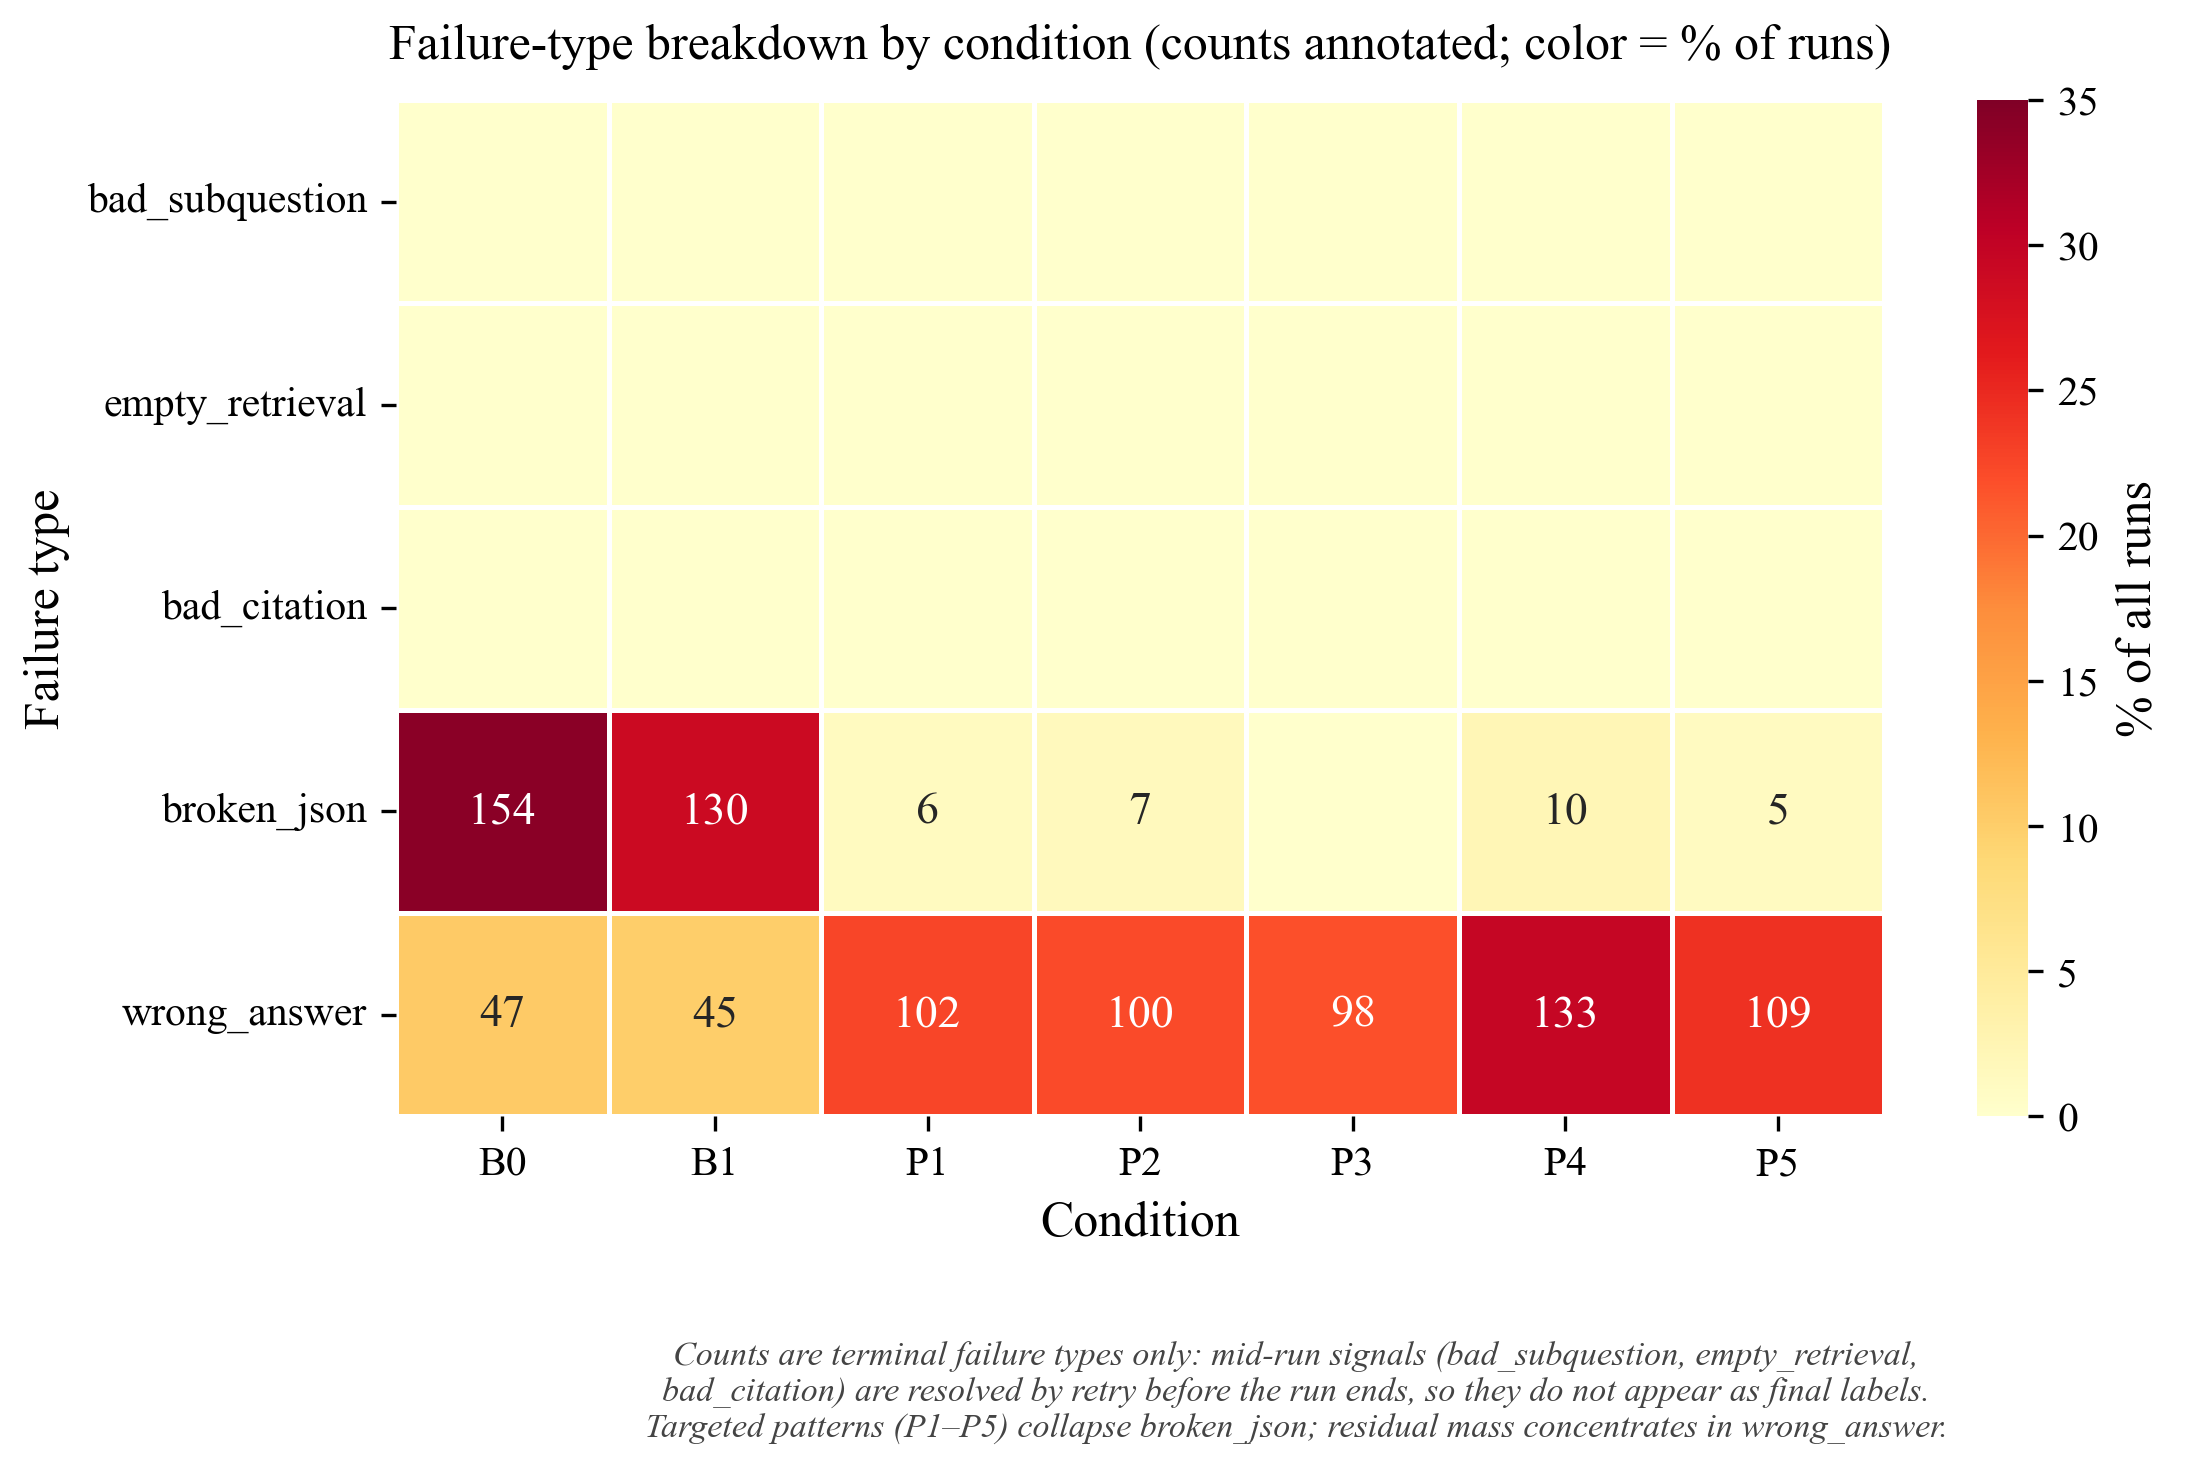
\includegraphics[width=0.92\linewidth]{figures/fig6_error_analysis.png}
  \caption{Terminal failure-type heatmap (\% of runs).}
  \label{fig:error}
\end{figure}

\subsection{Stage-failure heatmap}
\begin{figure}[t]
  \centering
  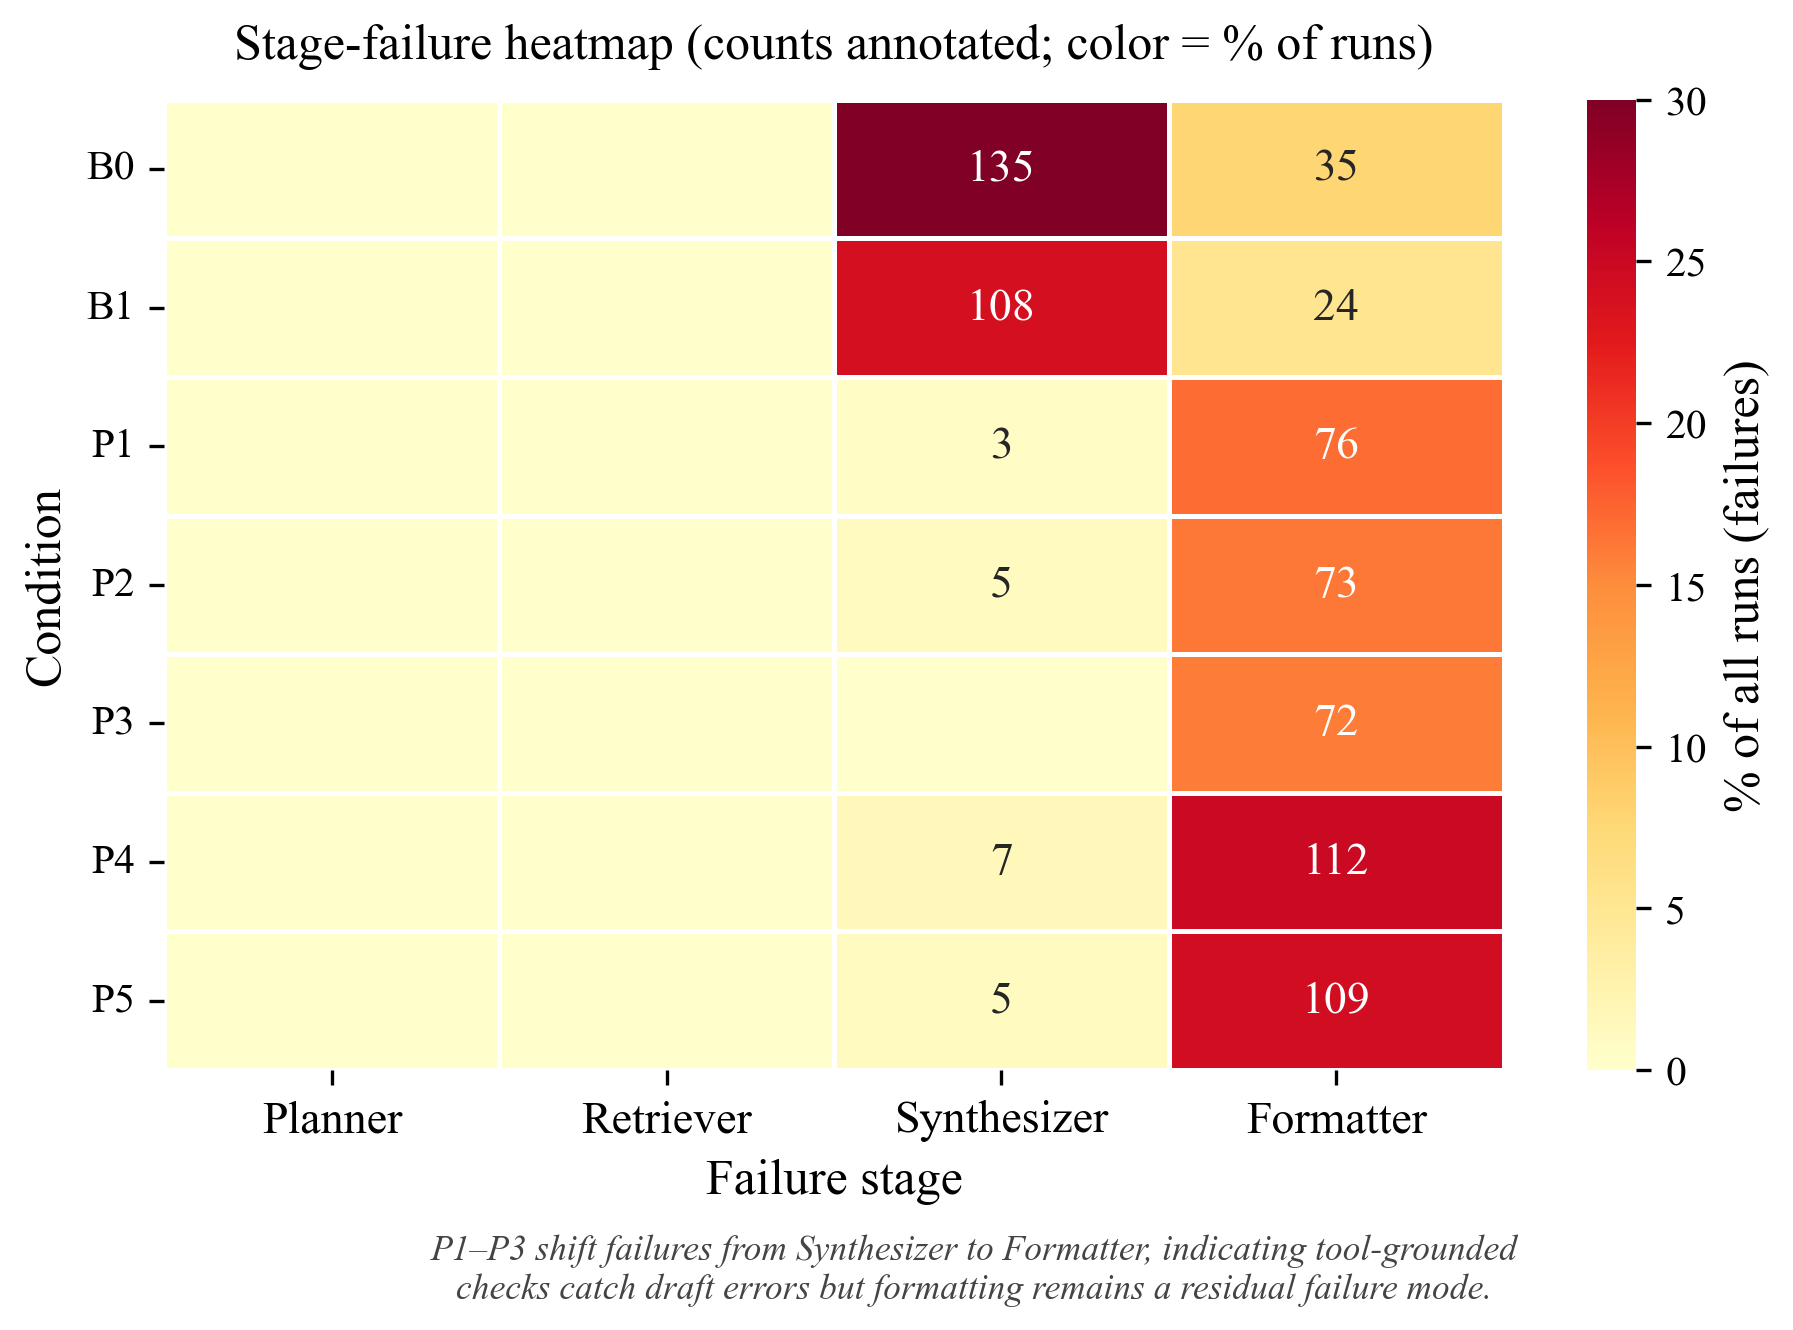
\includegraphics[width=0.92\linewidth]{figures/fig4_stage_heatmap.png}
  \caption{Stage-failure heatmap. P1--P3 shift mass from Synthesizer to Formatter.}
  \label{fig:stage}
\end{figure}

\subsection{2WikiMultihopQA validation}
\label{sec:2wiki}
B0/B1/P1/P3 on 50 2Wiki questions ($n{=}100$ runs/condition): ranking holds (P3 $+30$\,pp vs.\ B0, $p{\approx}1.6\times 10^{-5}$; P1 $+18$\,pp, $p{=}0.008$; B1 n.s.).

\subsection{GPT-4o-mini probe}
Same 50 Hotpot IDs ($n{=}100$/condition): B0 69\% (69/100; Wilson CI $[59.4\%, 77.2\%]$), P1 68\% ($-1.0$\,pp vs.\ B0, $p{=}0.879$), P3 71\% ($+2.0$\,pp, $p{=}0.758$). No significant lift over B0; baseline \texttt{broken\_json} is rare, so tool checks have little to repair.

\end{document}
